\chapter{Analyse des FIR-Filters}
\section{Aufgabenstellung}
Im zweiten Teil des Laborversuchs sollte das Verhalten des Filters mit den 
Ergebnissen der Vorbereitung verglichen werden.\\ Außerdem soll ein FIR-Filter 
h\"oherer Ordnung, mithilfe eines MatLab-Tools entworfen werden.
\section{Durchf\"uhrung}
Zur Analyse des in \ref{Cha:RealFIR} erstellten Filters wurde ein Sinussignal 
an den Eingang des Filters angelegt werden. Durch alternieren der Frequenzen des 
Signals, konnten wir dann die Nullstellen anhand der Amplitude des 
Ausgangssignals ermitteln.\\
Diese Analyse wurde dann mit Aufnahme des Amplitudenganges vertieft.\\
Zum aufnehmen der Sprungantwort wurde dann ein Rechtecksignal mit 2000Hz.
Diese Frequenz wurde ausgewählt, da ein zu schnelles Signal dazu führen würden, dass 
die Sprungantwort des Filters nicht in eine komplette Periode des Rechtecksignals passen 
w\"urde.\\\par
Im zweiten Teil dieses Versuchteils, wurde ein Filter h\"oherer Ordnung mit 
einem \gls{fda}-Tool entworfen. Dabei sollte folgende Parameter genutzt werden:
\begin{itemize} 
\item Equiripple-Charakteristik
\item Passband-Frequenz: 3400 Hz
\item Stoppband-Frequenz: 4000 Hz 
\item Abtastfrequenz: 48000 Hz 
\item Passband-Welligkeit: 2dB 
\item Stoppband-D\"ampfung: 80dB
\end{itemize}
\newpage
Die dadurch erzeugten Filter Koeffizienten wurden dann im fractional Format in 
die bereits vorhandene C-Header-Datei eingefügt. Dies ist in dem untenstehenden Quellcode-Ausschnitt zu sehen.\\
\begin{adjustbox}{width=\textwidth, keepaspectratio} 
  \label{code:procdataKompFIR}
  \begin{lstlisting}[title=process\textunderscore data\textunderscore KompFIR.c]
// Definition der Filterkoeffizienten
#define N_FILT 184 // Anzahl der Koeffizienten

const short coef[N_FILT] = {
       -5,    -12,    -25,    -43,    -67,    -98,   -132,   -168,   -200,
     -226,   -239,   -237,   -215,   -175,   -119,    -51,     21,     89,
      144,    179,    189,    173,    134,     79,     18,    -39,    -81,
     -100,    -92,    -59,     -7,     54,    112,    155,    174,    163,
      124,     64,     -5,    -69,   -115,   -132,   -114,    -64,      9,
       91,    164,    213,    224,    193,    124,     31,    -70,   -155,
     -206,   -209,   -160,    -66,     56,    181,    282,    334,    323,
      245,    112,    -52,   -214,   -336,   -390,   -355,   -231,    -36,
      196,    416,    575,    630,    555,    347,     33,   -336,   -686,
     -939,  -1017,   -864,   -454,    204,   1058,   2024,   2996,   3856,
     4500,   4843,   4843,   4500,   3856,   2996,   2024,   1058,    204,
     -454,   -864,  -1017,   -939,   -686,   -336,     33,    347,    555,
      630,    575,    416,    196,    -36,   -231,   -355,   -390,   -336,
     -214,    -52,    112,    245,    323,    334,    282,    181,     56,
      -66,   -160,   -209,   -206,   -155,    -70,     31,    124,    193,
      224,    213,    164,     91,      9,    -64,   -114,   -132,   -115,
      -69,     -5,     64,    124,    163,    174,    155,    112,     54,
       -7,    -59,    -92,   -100,    -81,    -39,     18,     79,    134,
      173,    189,    179,    144,     89,     21,    -51,   -119,   -175,
     -215,   -237,   -239,   -226,   -200,   -168,   -132,    -98,    -67,
      -43,    -25,    -12,     -5
};// Von MatLab generierte Filter Koeffizienten
  \end{lstlisting}
\end{adjustbox}

In Zeile 2 wurde die Anzahl der Koeffizienten festgelegt und in Zeile 4 bis Zeile 
26 wurden die Koeffizienten eingetragen, außer diesen \"Anderungen war es nicht 
notwendig den Quellcode anzupassen.\newpage


\section{Auswertung des Mittelwert FIR-Filter}
F\"ur diesen Aufgabenteil haben wir jeweils zwei 
Minimalf\"alle und zwei normale F\"alle ausgew\"ahlt, alle Eingangssignale haben eine Amplitude von 1V. Diese sind in Abbildung 
\ref{fig:5k1V} bis Abbildung \ref{fig:19k21V} 
\begin{figure}[H]
  \centering
    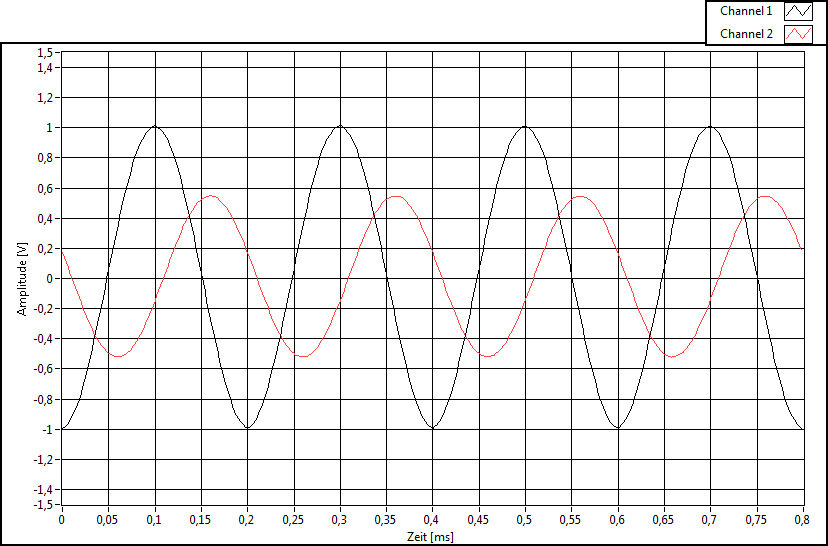
\includegraphics[width=\textwidth]{fir5k1VMax.png}
  \caption{Frequenz: 5 kHz}
  \label{fig:5k1V}
\end{figure}
In Abbildung \ref{fig:9k61V} und Abbildung \ref{fig:19k21V} sind die 
Auswirkungen der Nullstellen 
des Filters zu sehen. Dort ist das Ausgangssignal fast Null. In Abbildung \ref{fig:5k1V} 
und Abbildung \ref{fig:15k1V} ist zu sehen, dass das Signal ged\"ampft ist aber 
deutlich gr\"oßer Null ist.
Diese Ergebnisse entsprechen der Vorbereitung. \\\par
Die Verz\"ogerung zwischen Eingangssignal und Ausgangssignal ist, wie bereits im 
ersten Laborversuch, dem Versuchsaufbau zu verschulden, allerdings treten nun 
durch den Filter wiederum Verz\"ogerungen auf.
Diese Verz\"ogerungen sind damit zu erkl\"aren, dass der FIR Filter den Ausgang 
immer aus den letzten N\textunderscore FILT Werten bestimmt. Damit folgt auch das 
ausgegebene Signal diesem Muster.
\begin{figure}[H]
  \centering
    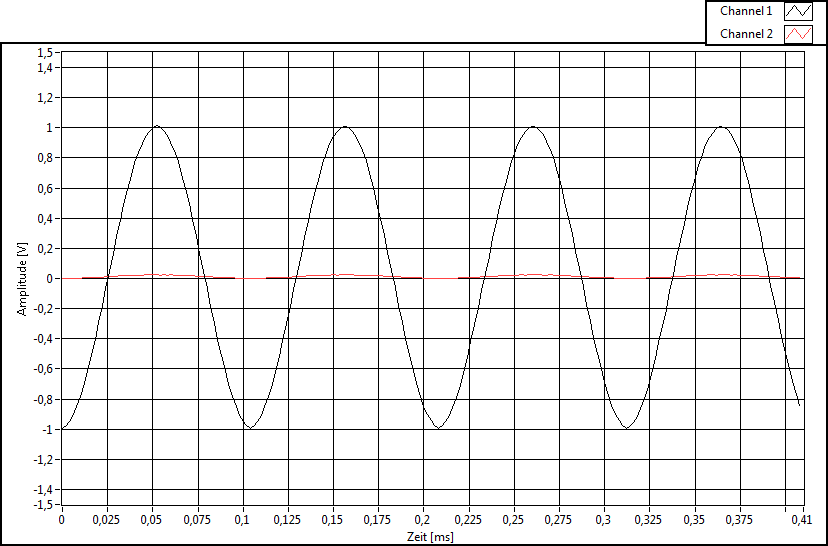
\includegraphics[width=\textwidth]{fir9k61VMin.png}
  \caption{Frequenz: 9,6 kHz}
  \label{fig:9k61V}
\end{figure}
\begin{figure}[H]
  \centering
    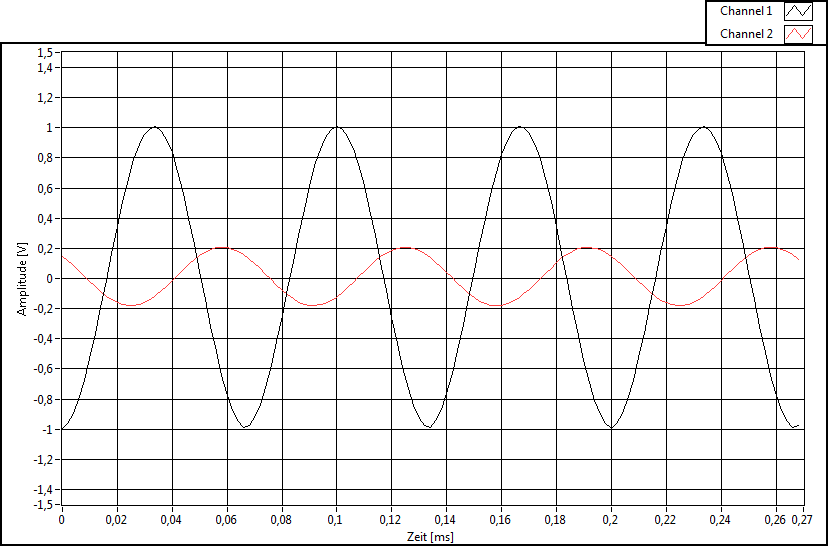
\includegraphics[width=\textwidth]{fir15k1VMax.png}
  \caption{Frequenz: 15 kHz}
  \label{fig:15k1V}
\end{figure}
\begin{figure}[H]
  \centering
    \includegraphics[width=\textwidth]{fir19k21VMin.png}
  \caption{Frequenz: 19,2 kHz}
  \label{fig:19k21V}
\end{figure}\newpage
Die Nullstellen lassen sich des weiteren im Amplitudengang ablesen, dieser ist 
in \ref{fig:AmpgangFIRMit} zu sehen. Dort ist bei ungefähr 9,6 kHz ein Einbruch 
auf -68dB und ein Einbruch auf -65dB bei 19,2 kHz zu sehen.\\
Auff\"allig, aber nicht weiter \"uberraschend, ist der Verlauf des Signals bei ca. 24 kHz. 
Dieser folgt aus dem Tiefpassverhalten des Codecs.
\begin{figure}[H]
  \centering
    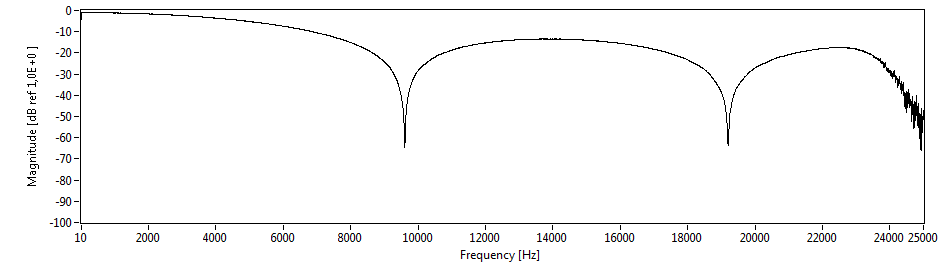
\includegraphics[width=\textwidth]{freqgang22_1.png}
  \caption{Amplitudengang des FIR Mittelwertfilters}
  \label{fig:AmpgangFIRMit}
\end{figure}
Im weiteren Verlauf soll nun die Sprungantwort des Filters analysiert werden.
\begin{figure}[H]
  \centering
    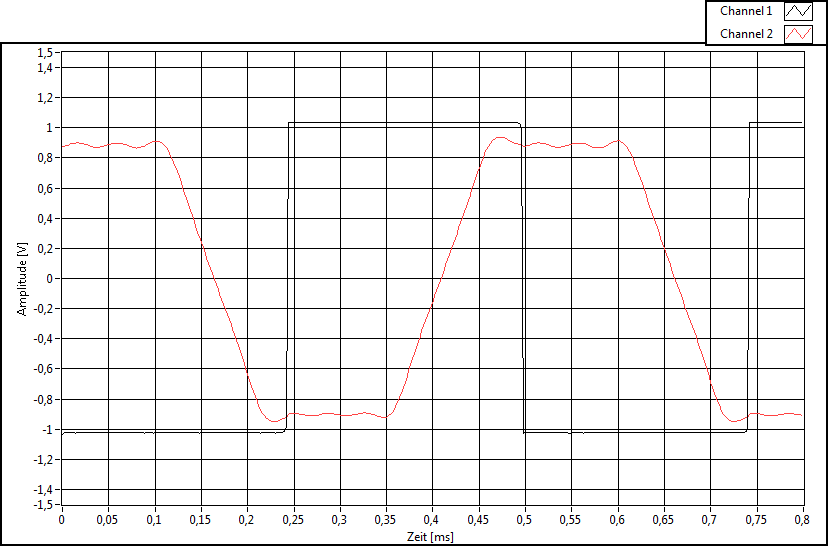
\includegraphics[width=\textwidth]{sq2k1v.png}
  \caption{Sprungantwort des FIR Mittelwertfilters}
  \label{fig:SprungFIRMit}
\end{figure}
Der Sprung ist mit dem schwarzen Graphen dargestellt und die Sprungantwort mit dem 
roten Graphen. Der lineare und leicht verzögerte Anstieg der Sprungantwort 
entspricht dem verhalten eines FIR Filter. In der Theorie m\"usste diese lineare 
Gerade eine Treppenform haben, diese Form wird allerdings durch das Tiefpassverhalten 
des Systems gegl\"attet. Wie bereits bei der Analyse der Ausgangssignale 
erw\"ahnt tritt eine Anstiegszeit von N\_FILT Werte auf, in diesem 
Beispiel sind dies 5 Werte, also 5 Abtastwerte. Damit lässt sich die 
Anstiegszeit berechnen.
\begin{equation}
  T_{rise} = N\_FILT * \frac{1}{f_{Abtast}}
\end{equation}
\begin{equation*}
%  T_{rise} = 5* \frac{1}{48 kHz} = 104,2\micro s
\end{equation*}
Diese Anstiegszeit deckt sich, mit leichter Abweichung, mit Abbildung 
\ref{fig:SprungFIRMit}.

\section{Auswertung des FIR-Filter h\"oherer Ordnung}
Das Matlab \gls{fda}-Tool erzeugt neben den Koeffizienten auch die Graphen 
welche das Verhalten des erzeugten Filters darstellen. Der ideale Amplitudengang des 
erzeugten Filters ist in Abbildung \ref{fig:MatlabAmpgang} zu sehen. 
\begin{figure}[H]
  \centering
    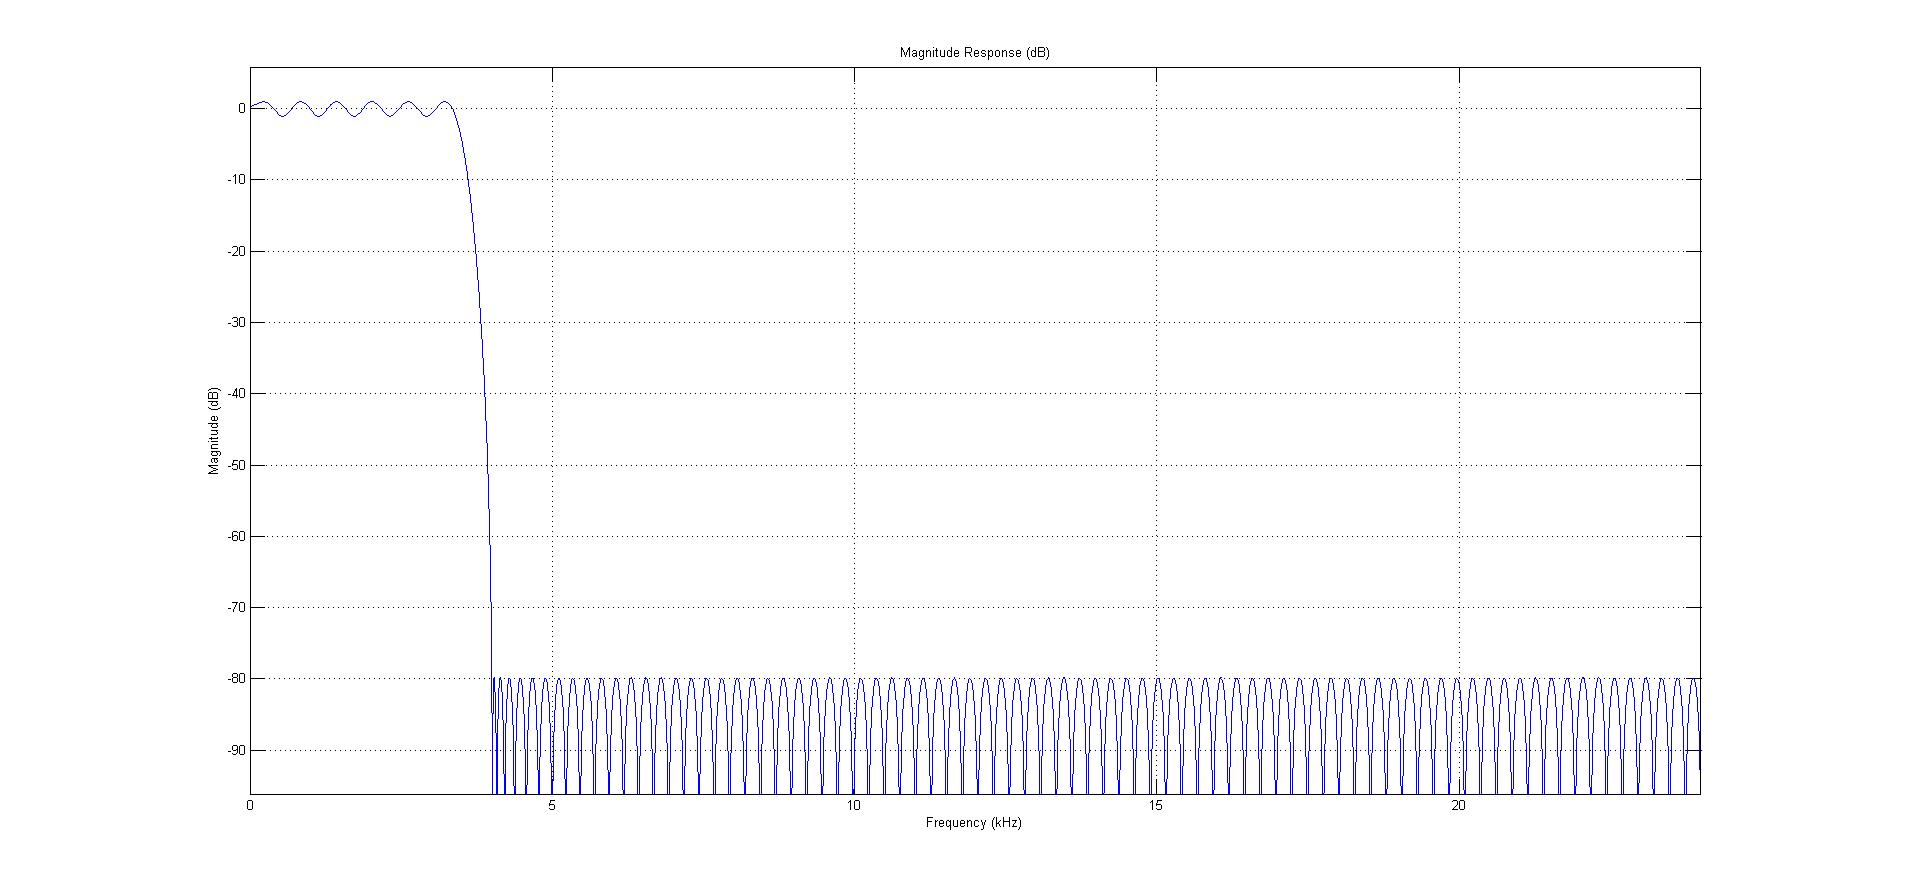
\includegraphics[width=\textwidth]{matlamplitudengang.jpg}
  \caption{Idealer Amplitudengang des erzeugten Filters}
  \label{fig:MatlabAmpgang}
\end{figure}
Im Vergleich dazu soll nun in Abbildung \ref{fig:DSPAmpgang} der reale Amplitudengang gezeigt werden.
\begin{figure}[H]
  \centering
    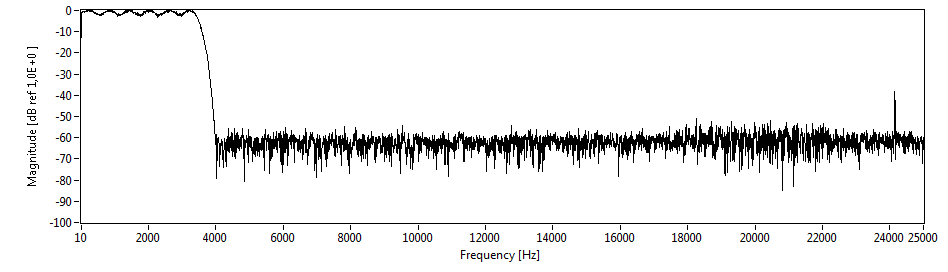
\includegraphics[width=\textwidth]{sqamplitudengang.png}
  \caption{Realer Amplitudengang des erzeugten Filters}
  \label{fig:DSPAmpgang}
\end{figure}
Beide Amplitudeng\"ange \"ahneln einander. Im Durchlassbereich ist im realen Amplitudengang eine leichte D\"ampfung zu erkennen. 
Diese liegt zwischen 1 dB und 2 dB und ist auf die Skalierung von ADC und DAC zur\"uckzuf\"uhren.
Die Grenzfrequenz betr\"agt in beiden Abbildungen ca. 4 kHz.\\
Im Sperrbereich ist deutlich zu erkennen das die D\"ampfung des idealen Amplitudengangs nicht erreicht wird. Es werden lediglich -60 dB erreicht, im idealen Amplitudengang sind es jedoch -80 
dB.\\\par

Die Sprungantwort des idealen Filters ist in Abbildung \ref{fig:MatlabSprung} und die Sprungantwort des realen Filters in Abbildung \ref{fig:DSPSprung} zu sehen.
\begin{figure}[H]
  \centering
    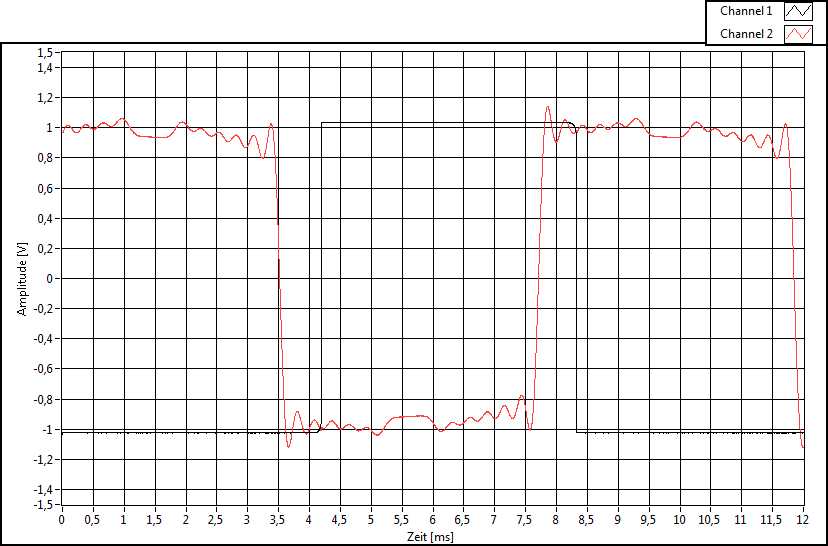
\includegraphics[width=\textwidth]{sq1201vfircomp.png}
  \caption{Reale Sprungantwort des erzeugten Filters}
  \label{fig:DSPSprung}
\end{figure}
\begin{figure}[H]
  \centering
    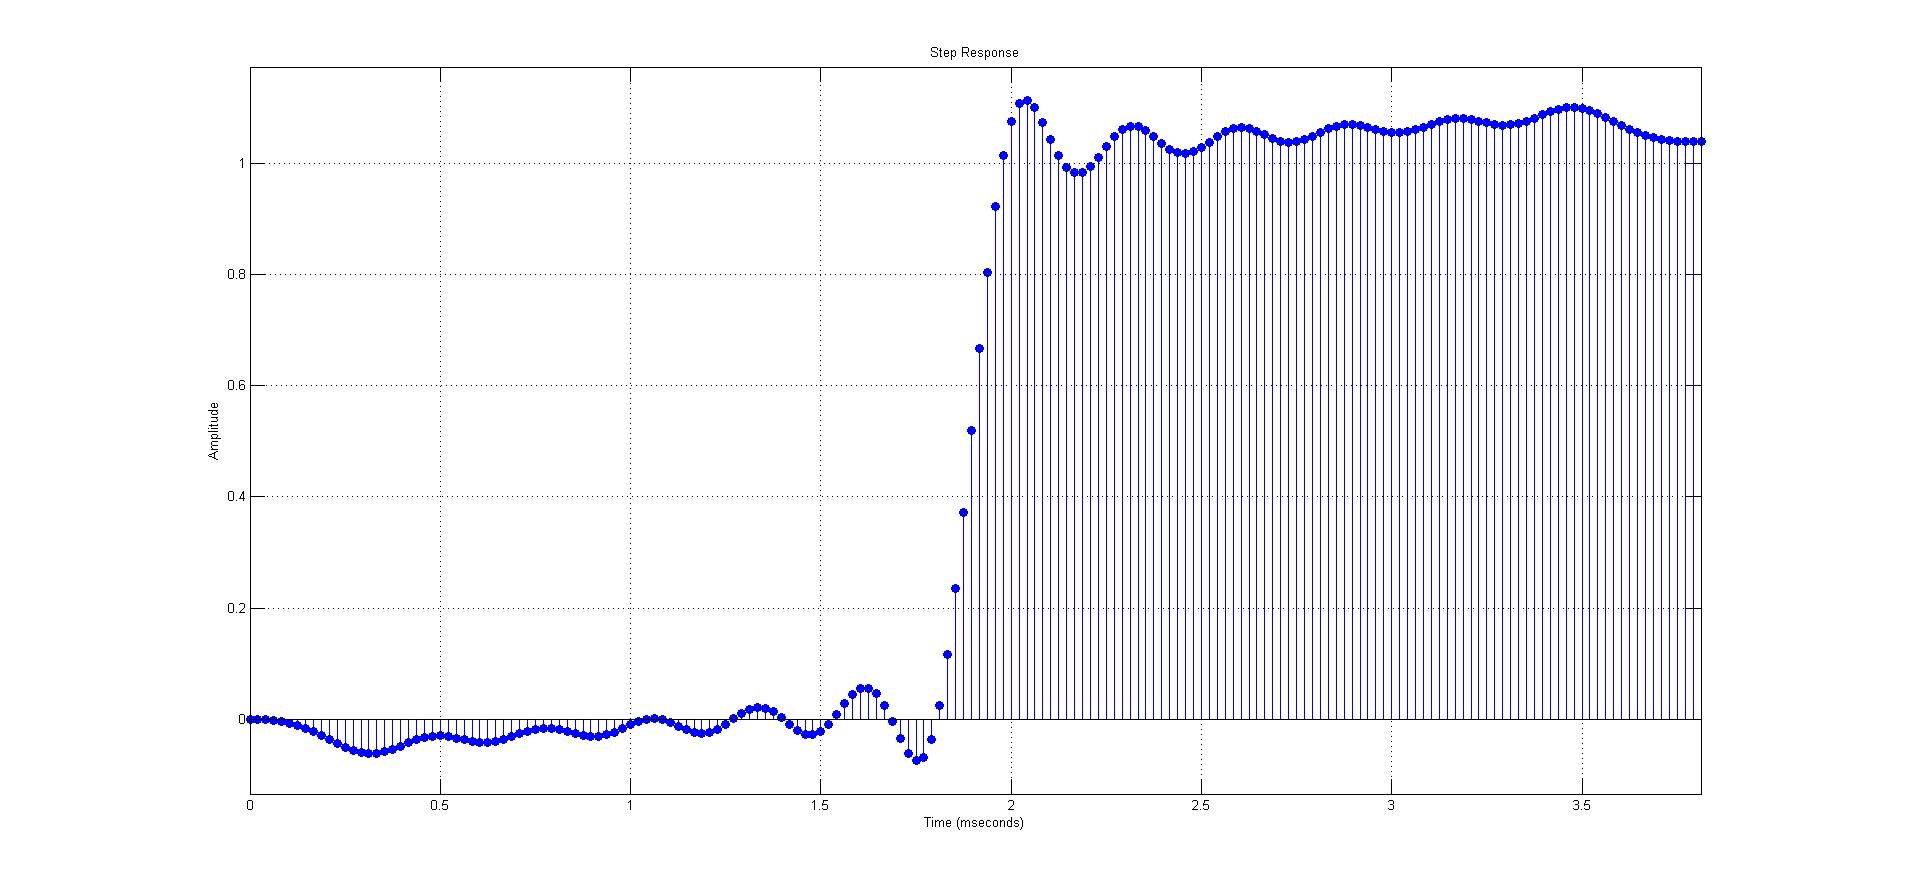
\includegraphics[width=\textwidth]{matlabsprungantwort.jpg}
  \caption{Ideale Sprungantwort des erzeugten Filters}
  \label{fig:MatlabSprung}
\end{figure}
Das Verhalten des realen Filters entspricht sehr genau unseren Erwartungen. Es ist lediglich eine leichte D\"ampfung zu erkennen.
Die Anstiegszeit, sowie das Überschwingverhalten sind fast identisch.